\section{Portalserver/ CMS-Systeme im Vergleich}
Das zuk�nftige Supportportal der PDV Systeme GmbH soll auf Basis eines Portalservers bzw. \ac{CMS}-Servers aufgebaut werden. Hierf�r werden im folgenden einige M�glichkeiten genauer betrachtet.

Ein Portalserver, welcher f�r das Projekt heran gezogen wird muss die folgenden Eigenschaften aufweisen.
\begin{itemize}
 \item Webseiten m�ssen frei gestalltbar sein
 \item Es muss die M�glichkeit bestehen Anwendungen f�r den Server zu entwickeln
 \item Das System muss Open-Source sein, um ggf. in den Quellcode eingreifen zu k�nnen
 \item Die Nutzer-Community sollte m�glichst gro� sein, damit Probleme leicht diskutiert und behoben werden k�nnen
 \item Der Server muss die M�glichkeit bieten Dateien zu verwalten, welche als Download oder Kontent in das Portal einflie�en
 \item Lauff�hing unter einer SQL-Datenbank wie MySQL oder MariaDB
\end{itemize}

Auf die Betrachtung reiner \ac{CMS}-System wird an dieser Stelle verzichtet, da diese nicht die gew�nschten Anforderungen eines Portalservers erf�llen.
Ein Vergleich verschiedener reiner \ac{CMS}-Systeme ist in der Bachelorarbeit "`Konzept und prototypische Implementierung eines �bergreifenden Dokumenten- und Medienmanagements"' zu finden.
\cite{Bachelorarbeit}


\subsection{Typo3}
Typo3 ist ein Verwaltungssystem f�r Internetseiten. Es basiert in der neusten Version 8.2 auf der PHP Version 7. 
Seit der Version 7.0 welche zugleich eine \ac{LTS} Version ist, wird es unter dem Namen Typo3 \ac{CMS} vertrieben. 
\cite{WikiTypo3}

\begin{figure}[!ht]
\centering
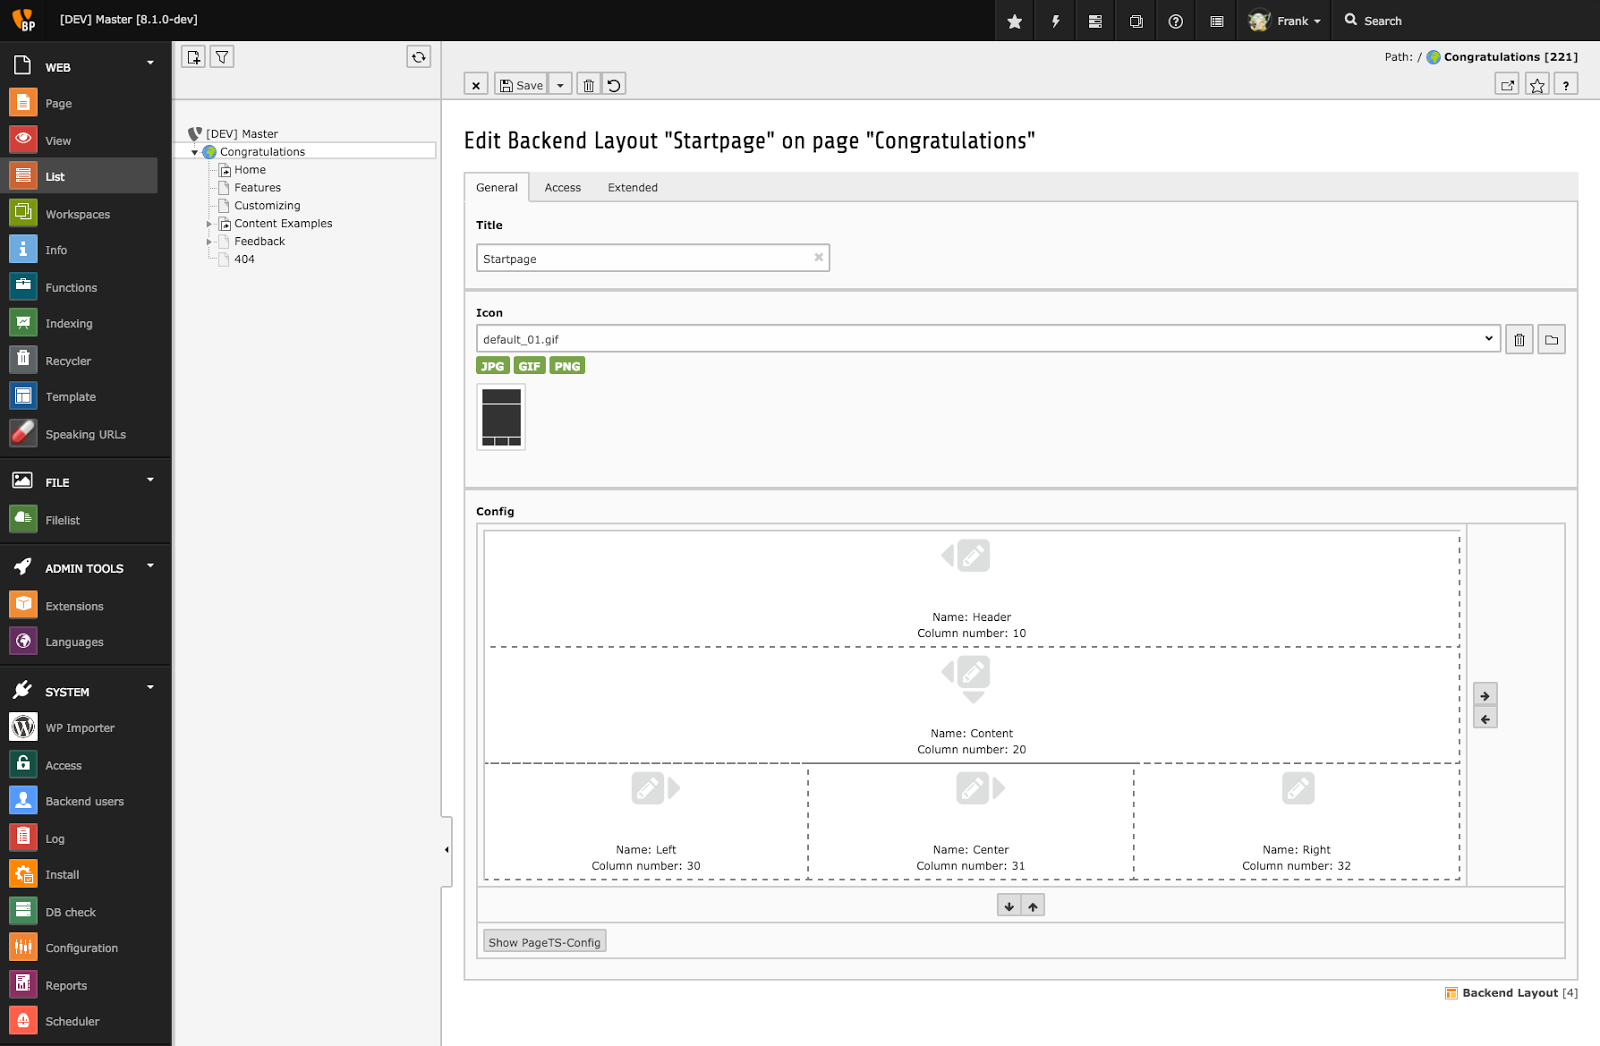
\includegraphics[width=16cm]{Bilder/Typo3_Backend.png}
\caption{Typo3 Backend im Seitenbearbeitungs Modus \cite{Typo3Bild}}
\label{Typo3_Backend_Bild}
\centering
\end{figure}

Es ist m�glich unter Verwendung von PHP, Extbase und Fluid eigene Erweiterungen f�r den Portalserver zu entwickeln. Die jeweiligen Erweiterungen wirken im Fronten von Typo3 wie ganz normale Webseiten.
Auf Extbase und Fluid wird im Kapitel \ref{Typo3} genauer eingegangen.

Ein Vorteil von Typo3 ist, dass es eines der am h�ufigsten verbreiteten Portalserver auf dem Markt ist. Selbst gro�e Firmen wie "`Sixt"' setzten auf Typo3 bei der Erstellung ihrer Internetportale.
Durch die gro�e Verbreitung von Typo3 ist auch die Community um die Software sehr gro� und man findest schell zu fast jedem Problem im Internet eine L�sung.

Typo3 kann im Zusammenspiel mit MySQL, MariaDB, PostgreSQL oder Oracle als Datenbank betrieben werden. Nur mit Hilfe einer dieser Datenbank im Hintergrund ist Typo3 stabil Lauff�hing und kann produktiv eingesetzt werden.

Durch ein �bersichtliches Backend (siehe Abbildung \ref{Typo3_Backend_Bild}), ist es auf f�r Laien m�glich qualitativ Hochwertige Webseiten zu erstellen, ohne viel Kenntnis von Webtechnologien wie HTML oder CSS zu haben.

Ein Upload von Dateien f�r den Download beziehungsweise als Seiten-Kontent ist ebenfalls unter Typo3 m�glich. Zus�tzlich dazu ist es m�glich das Nutzer Dateien auf den hochladen. 
Hierdurch entsteht auch die M�glichkeit ein Austauschportal f�r Dateien zu schaffen. Nutzer k�nnen so in einer sicheren Umgebung sensible Daten untereinander oder mit Mitarbeitern austauschen.
\cite{LobacherTypo3}

\subsection{Typo3 Neos}
\subsection{Joomla}
\subsection{Drupal}
\subsection{Auswertung der m�glichkeiten}
\section{Typo3}\label{Typo3}
\subsection{Typo3 8.2}
\subsection{Extensions}
\subsection{TypoScript}
\subsection{Fluid}
\section{Modulare Extensions}
\section{Neue Webtechnologien}
\subsection{Google Polymer}
\subsection{AngularJS}
\subsection{HTML5}
\subsection{CSS3}
\subsubsection{Bootstrap}
\subsubsection{MaterializeCSS}
\subsection{PHP7}
\subsection{Google Dart}
\section{Zusammenspiel der Technologien}
\section{Zusammenfassung}
\section{Fazit}